\section{Architecture}

\begin{figure}[h!]
  \centering
  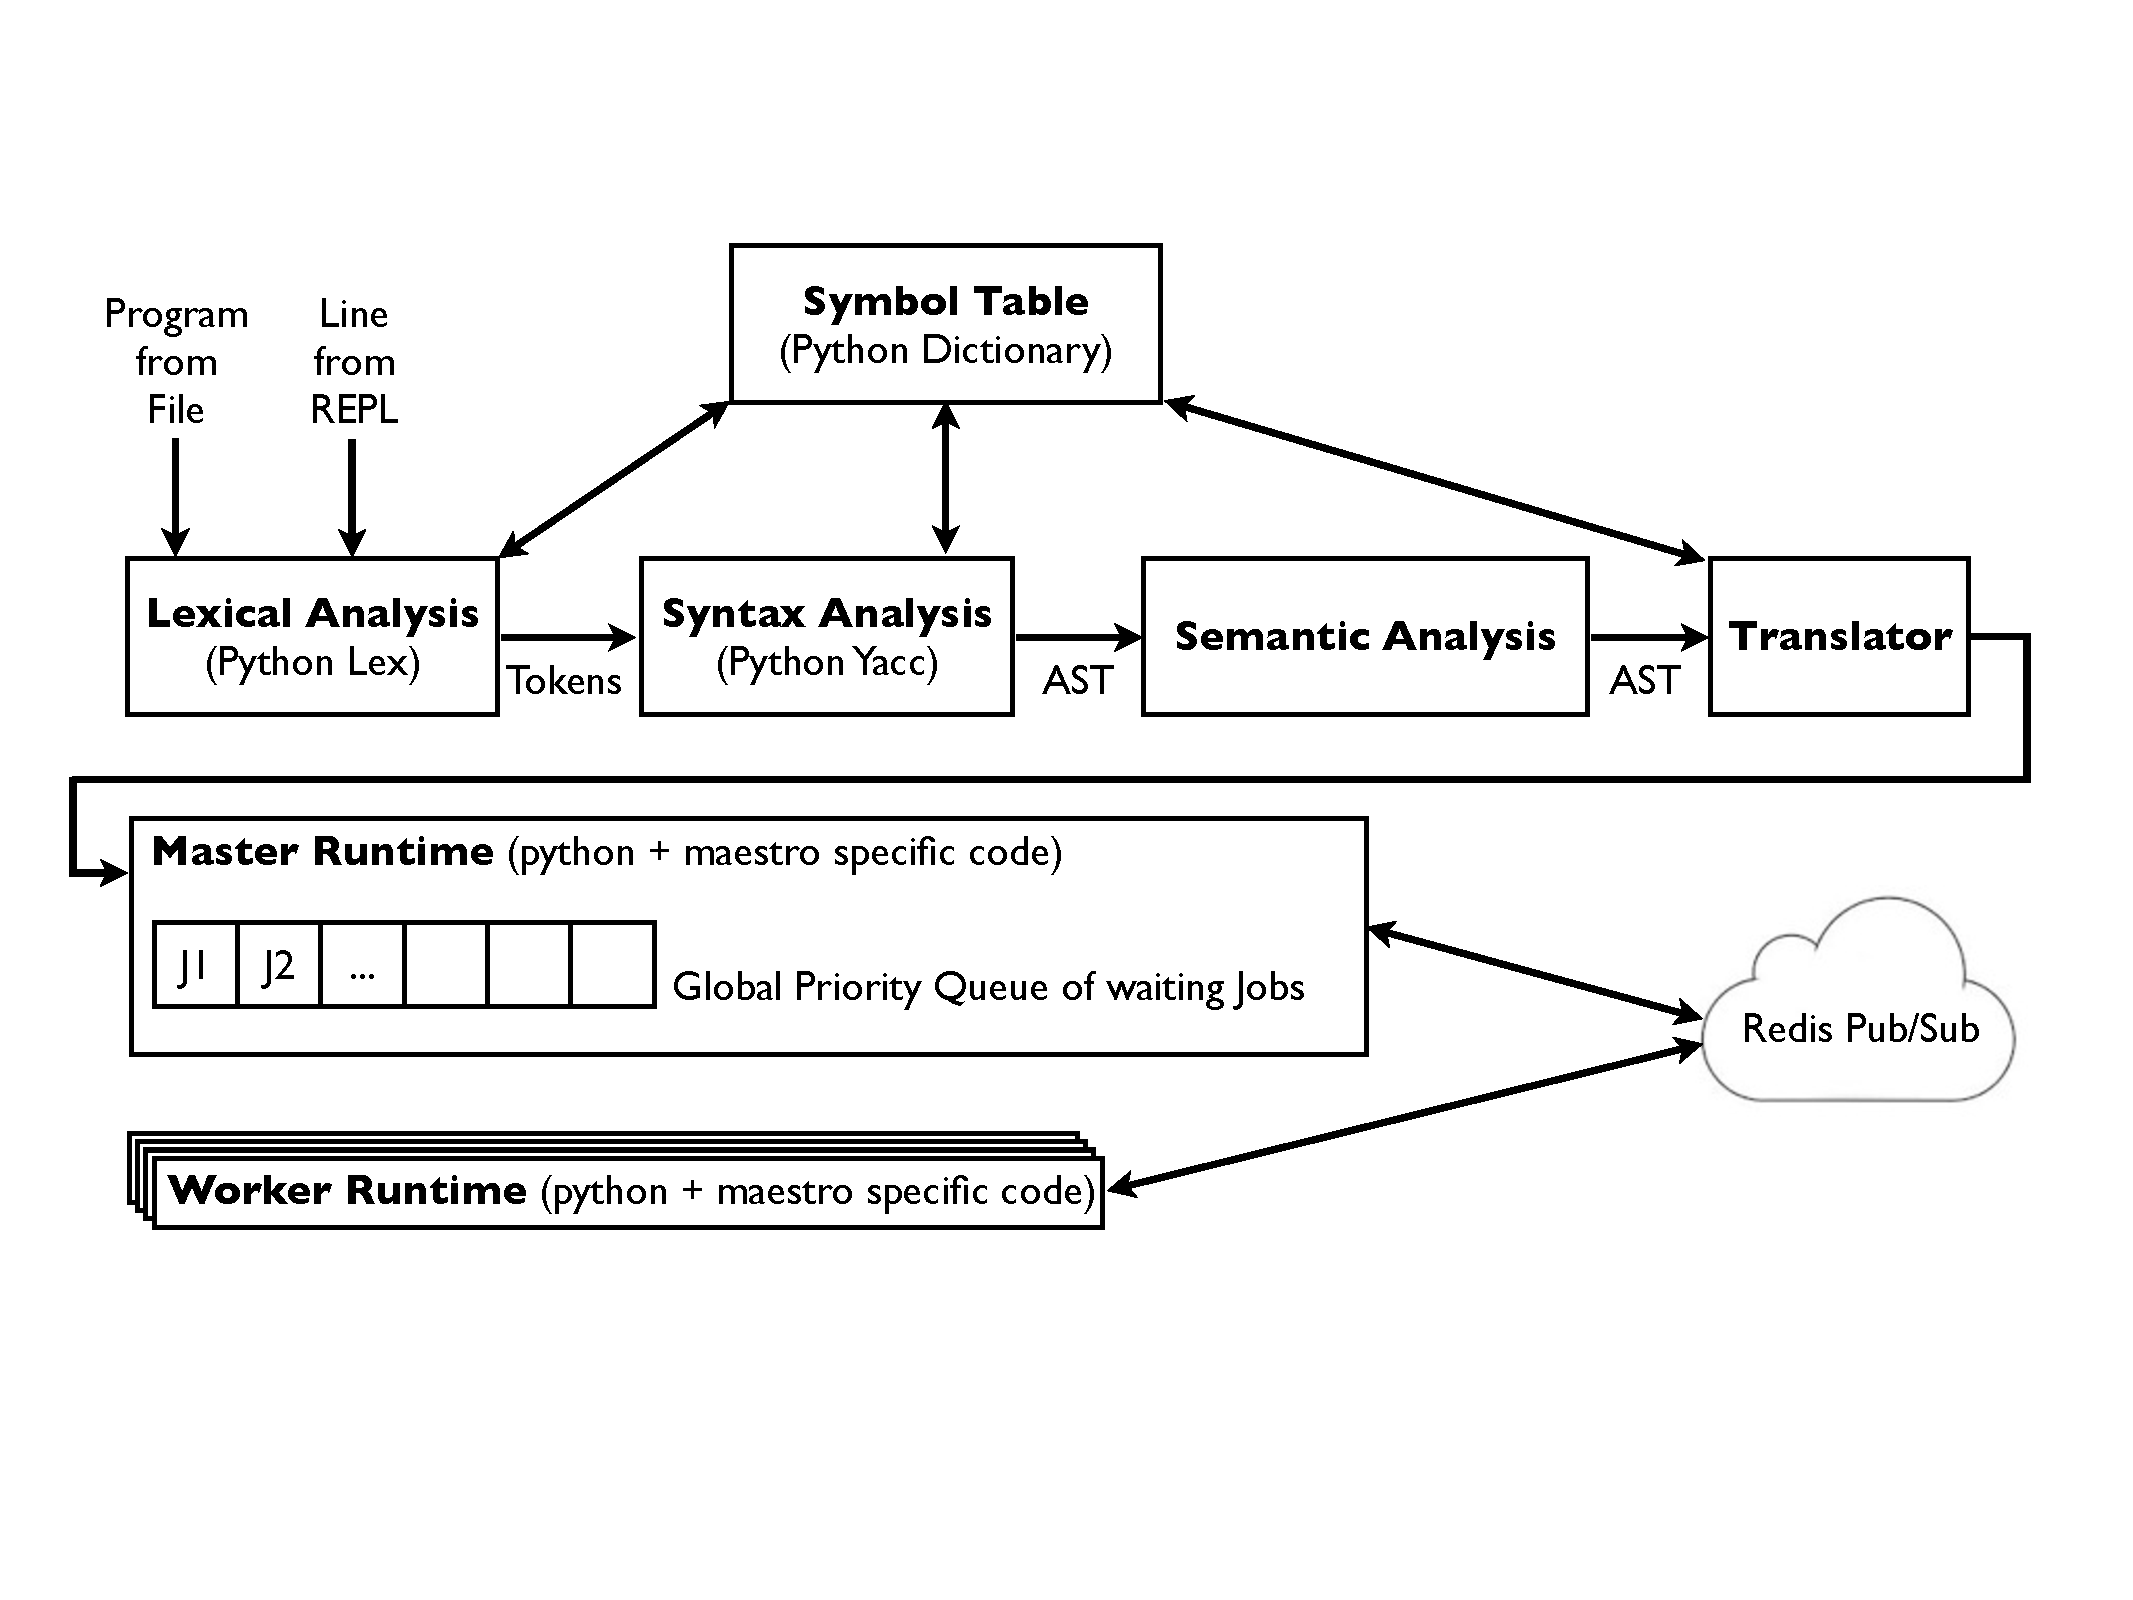
\includegraphics[width=15cm]{figures/archi.pdf}
  \caption{Maestro Architecture}
\end{figure}

\subsection{Interfaces}

\subsection{Modules}
Describe the interfaces between the modules.\\

State which modules were written by which team members.

\paragraph{Lexer (Mathias)}:
\paragraph{Syntax Analyser (Mathias)}:
\paragraph{Semantic Analyser (Georgios)}:
\paragraph{Translator (Mathias)}:
\paragraph{Backend (Vaggelis)}:
\paragraph{Testing (Arun and Yiren)}:

\section{Orgnaisation}
The hard thing with a multi-person project with many interacting parts is to figure out a way to all work in parallel.
We also wanted an early "hello world"...

To best achieve these objectives, 
